\documentclass[11pt]{article} % use larger type; default would be 10pt
\usepackage{graphicx,amsmath} % support the \includegraphics command and options
\usepackage{color}

\newcommand{\andyc}[1]{[{\color{red}\sc Andy says: {\tt #1}}]}
\newcommand{\scotlandc}[1]{[{\color{red}\sc Scotland says: {\tt #1}}]}
\newcommand{\lucasc}[1]{[{\color{red}\sc Lucas says: {\tt #1}}]}
\newcommand{\xinranc}[1]{[{\color{red}\sc Xinran says: {\tt #1}}]}
\newcommand{\yuhyunc}[1]{[{\color{red}\sc Yuhyun says: {\tt #1}}]}
\newcommand{\ianc}[1]{[{\color{red}\sc Ian says: {\tt #1}}]}
\newcommand{\marcosc}[1]{[{\color{blue}\sc Marcos is confused and says: {\tt #1}}]}

\oddsidemargin=0.25in
\evensidemargin=0.25in
\textwidth=6in
\textheight=8.75in
\topmargin=-.5in
\footskip=0.5in

\title{Nearest-Neighbor Matchup Effects:  Accounting for team match ups in the NCAA tournament}
 \author{The Lemanski Sports Analytics Group}        
\begin{document}
\maketitle
\section*{Task Summary: First round of composition Due June 13\\
Final Manuscript Due July 15}

Current Assignments:
\begin{itemize}
\item Lucas - Luck
\item Xinran - Popular Methods
\item Marcos - Recommendations, Decision Theory
\item Ian/Yuhyun - Lit Review - Introduction
\item Andy : Modeling, Evaluation, Data, Discussion
\end{itemize}

\andyc{I thought it might be worthwhile to put a list of papers to incorporate as reference.  Ian and Yuhyun are likely working on something similar.}\\
Articles to incorporate (likely include solid list of references themselves):
\begin{itemize}
\item \cite{cattelan2013}: An application of dynamic Bradley-Terry model that allows team strength to vary of course of tournament.  Also has a fruitful list of references.
\item \cite{Kvam2006}: An overview of the logistic regression Markov Chain (LRMC) method for prediction.  A good read, which also contain useful citations.
\end{itemize}


\section{Introduction}
 Every March, millions of people take to an American tradition, filling out an NCAA tournament bracket.  Typical strategies include listening to so-called experts or following one's intuition, although the rise in sports analytics and the popularity of sites such as Nate Silver's fivethirtyeight.com are increasing the use of data-driven methods.  With this work we review analytic approaches to forecasting NCAA tournament games and introduce our modeling framework designed to capture matchup effects.   Many common methods for predicting outcomes assess overall team strength using ranking based metrics.  In addition to quantify overall team strength, our methodology provides a data-driven approach to assess team by team match ups and address statements of the form: \emph{"Team Y is a tough draw for team X due to their tempo, size, athleticism, three point shooting, ect.."}.  The essence of of the matchup effects is to discern the existence and magnitude of team-by-team match ups.  While there certainly is a high degree of uncertainty involved in predicting outcomes and a small number of games for evaluation, we demonstrate the efficacy of our matchup effects.  We predicted Duke would lose.  THE END
\subsection{Common Prediction Methods}
Many commonly used methods or models include a seeds based approach or using one of several rankings systems: Sagarin, Pomeroy, ESPN BPI, ect..
\subsection{Other}We should be explicit about the Kaggle comp. vs. just filling out a bracket. For kaggle, there are no broken brackets.
\subsection{LitReview}
Literature Review: What people have done for predicting tournaments before (both bball and other sports are fine), March madness in general (how many people watch, how much revenue is it worth). Predicting human performance in sports (it's hard), history of Kaggle.

%%%%%%%%%%%%%%%%%%%%%%%%%%%%%%%%%%%%%%%%%%%
\section{Data}
The key component to any successful analytic approach is quality data.  For those predicting NCAA basketball games, a plethora of data is available. While tidbits like \emph{Duke is undefeated in the first round of the tournament on even years when playing a team from the state of Georgia} might be entertaining for television viewers they are nonsensical for prediction.  In fact, this particular one would no longer hold after Mercer's upset of Duke this year. Nevertheless, some components with predictive power such as wins, losses, NCAA tournament seedings as well as many common rating systems can easily be obtained. Other factors such as strength of schedule, free throw percentage, and team tempo require more work for collection and analysis. Given the volume of data and the multitude of ways it can be aggregated and used, the question is what aspects are high quality predictors of tournament outcomes? We break the data into two segments: influential factors and rankings. First we provide a description of influential factors for basketball prediction. Then an overview of common ratings metrics which incorporate many of the influential factors will be displayed. In our experience, unsurprisingly, these rating systems perform quite well.

\subsection{Influential factors} 
There are many influential factors for predicting college basketball games and NCAA tournament game in particular. We first start with game level data that has been aggregated to reflect team characteristics. A few of these are self explanatory, such as winning percentage and average point differential. Winning percentage and average point differential are largely a function of opponents played, but still provides a nice description of overall team strength. Hence, some metric assessing and controlling for the strength of competition is also prudent. Other useful factors include team height, free throw percentage, percent of points scored on three pointers. Another important factor is home court advantage which is consistently shown to be worth about 4 points (\cite{harville1994}).  

Many other traditional, aggregated stats such as points scored, rebounds, and turnovers would appear to be useful, but are  tempo dependent. For instance, a team with a very quick pace will tend to have more rebounds than one that plays slower. This doesn't mean that the quicker pace team is a better rebounding team, given the larger number of rebounds available to be had. A simple adjustment would be to use offensive and defensive rebound percentage - that is the percent of available offensive and defensive rebounds a team collects. Similarly points scored and points allowed are adjusted to control for the total number of possessions a team has during a game.  Ken Pomeroy defines adjusted offensive efficiency and adjusted defensive efficiency as the number of points scored or allowed over 100 possessions (\cite{kenpom.com}.)

\subsection{Common Ratings Components} The purpose of using the influential factors is to construct a metric for overall team strength. An alternative possibility is to use one or more of the preexisting rating systems. With the large number of people working in this area, Ken Massey's website www.masseyratings.com contains nearly 70 different systems, it is no surprise that the best of these rankings work quite well and we have found it difficult to make major improvements over these ranking systems. While some of the algorithms are proprietary, we provide an overview of the main points for select algorithms.\subsubsection{NCAA Tournament Seeds}
Currently, the NCAA selection committee selects 36 teams in addition to the 32 teams conference champions and places the 68 teams into brackets for the NCAA basketball tournament. The seeding system, which rates teams one through sixteen in each region - not including the teams in the play in game - is well known. A lesser known rating is the so called `S-curve' which gives an ordinal ranking of each team in the field.  
\subsubsection{Logistic Regression / Monte Carlo}
The Logistic Regression / Monte Carlo (LRMC) method detailed in (\cite{Kvam2006} and \cite{mark2010}) is a two step procedure used to produce ordinal rankings of each team. The first step evaluates every game played during the season to compute the probability that the winning team is better than the losing team. This step uses the score at the end of regulation (e.g. overtime results are not included) and the home team in a logistic regression setting. The second step uses these probabilities in a Markov chain to produce the ordinal rankings. Specifically, each team is given a state in the chain based on the head-to-head probabilities and the ordinal ranking is a result of the ordering for the steady state probabilities of the chain.

\subsubsection{RPI}
The most well known rating system may very well be the Ratings Percentage Index (RPI). The RPI was created in 1981 as a tool for evaluating teams for admission and seeding to the NCAA basketball tournament. The RPI calculation uses three components, Winning Percentage (WP), Opponents Winning Percentage (OWP), and Opponents Opponents Winning Percentage (OOWP), with weights specified as:
\begin{eqnarray*}
RPI = \frac{WP}{4} + \frac{OWP}{2} + \frac{OOWP}{4}.
\end{eqnarray*}
The RPI is often criticized for heavy reliance on winning percentage and failure to account for other indicators such as point differential that illuminate the team strength.

\subsubsection{Sagarin}
Another well known ratings system is Jeff Sagarin's computer ranking system, known simply as the Sagarin rankings. Sagarin rankings are a staple, because of both the longevity  - they have been used since 1985 - and the quality. The exact methodology is unknown, but the Sagarin rating is actually a composition of three separate models. One model uses only wins or losses without regard to point differential, while the other two focus primarily on point spreads. A characteristic of the Sagarin rankings is that difference in the team ratings represents the expected point spread for that matchup on a neutral court. For the 2013-2013 year the home court advantage is estimated as 3.38 points (\cite{sagarin}).
\subsubsection{Pomeroy}
The Pomeroy rankings are issued by Ken Pomeroy and largely driven by the Pythagorean Expectation, a formula developed by Bill James for baseball prediction (\cite{james}).  A theoretical derivation of the Pythagorean Expectation using a Weibull distribution \cite{miller2007}. The Pythogorean expectation is
\begin{eqnarray}
E[Pr(Win)] = \frac{\text{points scored}^c}{\text{points scored}^c + \text{points allowed}^c},
\end{eqnarray}
where points scored and points allowed are season totals and $c$ is a constant, Pomeroy uses 10.25.  Rather than actual points scored Pomeroy uses adjusted and defensive efficiencies as inputs to the Pythogorean expectation, which gives an average error of 8.25 points based on backtesting.  On a related note, on his website \cite{kenpom.com2} states:
\begin{quote}
I don't think you can come up with a prediction method that will have an error of less than eight points. And if you can, don't tell anyone! Because that would be a really good system. That should also tell you a lot about why it's difficult to anticipate what will happen in a single contest between teams. It's also a good illustration of the large role randomness in any single game. So even if you know it all, you can't possibly know it ALL.
\end{quote}
This quote illustrates the difficulties inherent in basketball prediction. Later in the manuscript we discuss the effect of luck in the NCAA tournament and bracket prediction contests. This format certainly is not conducive for identifying the \emph{best} team, but it is quite entertaining. \andyc{move this quote up to introduction: section on prediction?}
\subsubsection{Rating Comparison}
The most popular ranking systems may be the Associated Press and Coaches top 25 polls, which aggregate votes by coaches or media members. Unfortunately, votes are only tallied for the top 25 teams on each ballot; hence, they are incomplete and not considered here. Table \ref{tab:ranks} contains pre-tournament rankings for the top 16 seeds in the NCAA tournament as well as the eventual national champion Connecticut, who was a 7th seed and 26$th$ in the S-curve.
\begin{table}[h!]
\caption{Pre-tournament Ranking Comparison}
\footnotesize
\centering
\begin{tabular}{l|ccccc|c}
  \hline
  \hline
 Team & Sagarin Rank &  Pomeroy Rank & RPI & LRMC Rank & Seed& Ave. Rank  \\ 
  \hline
 Arizona         & 1  &1    & 2     & 2 & 2& 1.6  \\
 Florida          & 3  &3    &1      &3 & 1& 2.2\\
  Kansas         & 6  &8    & 3    & 4& 7 &5.6\\
 Virginia         & 5  &4     &8    &8 & 4 &5.8\\
 Wichita St    & 12 &5      & 4    &5 & 3 &5.8\\
 Villanova      & 4  &7    & 5    & 9 & 5 &6\\
 Duke             & 7  &6     &9     &6 &9&7.4\\
 Louisville      & 2  &2    & 19   & 1 &13 & 7.4\\
  Creighton &  11 &   9 & 10   &7 &11& 9.6\\ 
 Wisconsin  &   9   &13   & 6   &  11 & 8 &9.4\\
 Michigan & 10 & 15& 11& 16& 6 &11.3\\
 Michigan St & 8  &10   & 18 & 12& 14&12.4\\
 UCLA & 15& 18& 14&10 &15 &14.4\\
 Iowa St &13 &23  &7 &19 &12 &14.8 \\
 Syracuse &19 &14  &16 &24 &10 &16.6 \\
 San Diego St&22 &21  &15 &25 &16 &19.8 \\
  \hline
  Connecticut & 24& 26& 22&26& 26&24.8\\
  \hline
   \hline
\end{tabular}
\label{tab:ranks}
\end{table}
There are some similarities but each of the ranking system has its own flavor.
\section{Popular Methods}  This section provides a review of several existing methods for tournament prediction.
\subsection{Rating Based Methods} 
The seeds and ratings discussed earlier contain implicit or explicit means for tournament prediction.  For instance the Sagarin rankings are designed to reflect the point spread between two teams, incorporating a term for the variance of the outcomes under a Bayesian framework provides an efficient way to compute winning probabilities.  Similarly for Pomeroy, ESPN BPI, coefficients for predicting point spreads or in a binary regression can be computed.
\subsection{Ensemble Methods}
Combining the ratings from several different sites is a popular strategy.  In fact this is the technique used by Nate Silver's 538 methodology?
\subsection{Wisdom of the Crowds?}
Another popular option would be to use the \emph{Wisdom of the Crowds}.  ESPN provides a mean probability across every bracket submitted to the site.
\scotlandc{include all into sensitivity study with Lucas}

\subsection{Evaluation}
\andyc{Xinran's piece here}


\section{Decision Theory - Optimal Strategies}
Suppose we have estimates of predictive probabilities for the outcomes of all possible matchups in the NCAA tournament. Decision theory gives us a framework to choose the optimal submission for almost any bracket competition. 

ESPN's yearly tournament challenge draws millions of March Madness fans into bracket competitions, or pools, with their friends. In some cases, these pools wager a certain amount of money, and the highest-scoring bracket wins the jackpot. Additionally, ESPN offers some prizes for the best brackets over all submissions. Most players are therefore keen on entering such competitions with a bracket that is likely to win. 

The ESPN Tournament Challenge awards points for each matchup according to the formula $10\times2^{r-1}$ where $r$ is the round in which the matchup occurs. So a correct pick for the third round will give $40$ points. Scoring is clearly done in this way so that each round has the potential of awarding a player the same number of points: 320. 

Recently in the headlines, Warren Buffet announced a prize of $\$1$ billion for the first perfectly-predicted March Madness bracket. Predicting a perfect bracket is similar to the ESPN tournament challenge in that the optimal choice requires an understanding of the underlying probabilities governing matchups between two teams. Ultimately the competitor will need to search through a discrete space to find an optimal submission. Niemi et al. (2005) also suggest using a contrarian approach to bracket selection for the ESPN challenge in order to set a submitted bracket apart from other similar brackets within the same pool. 

In general, even given the true probabilities of all possible matchups among the 64 teams in the tournament, selecting an optimal submission is not a simple problem. Suppose that in a strange year, only four teams qualify for the NCAA tournament -- teams A, B, C, and D. Further, suppose that teams A and C are number 1 seeds, so that they will respectively play against teams B and D in the first round. Table \ref{tab:hypothetical} shows possible probabilities for the outcomes of all six possible matchups. Notice that picking the highest probablity outcome at each round will give a bracket with likelihood $0.6\times0.8\times0.1=0.048$. However, picking the underdog between teams A and B will give a bracket with likelihood $0.4\times0.8\times1=0.32$. 

Clearly, the latter bracket is the highest-likelihood bracket, which illustrates the point that brackets ought not to filled out round-by-round. This motivates underdog picks and highlights the fact that the optimal process for bracket selection is not always obvious.

\begin{table}
	\centering
	\begin{tabular}{|cc|c|}
		\hline
		Team 1	&	Team 2	&	Probability of Team 1 beating Team 2 \\
		\hline
		A 		&	B 		&	0.6\\
		A 		&	C 		& 	0.1\\
		A 		& 	D 		& 	0.1\\
		B 		&	C 		&	1\\
		B 		& 	D 		&	1\\
		C 		& 	D 		& 	0.8\\
		\hline
	\end{tabular}
	\caption{\label{tab:hypothetical}}
\end{table}

\subsection{Kaggle Competition}

The Kaggle competition is scored based on a log-loss function. Submissions consist of a list of probabilities that determine the outcomes of all 2,278 pairwise matchups between the 68 teams admitted into the March Madness playoffs. Only the 63 matchups that occur during the tournament end up in the calculation of the loss function.

Suppose a competitor in the Kaggle competition is confident in her ability to estimate the probabilities of pairwise outcomes. Is it optimal, therefore, for her to submit these predicted probabilities? Or is there a benefit to adjusting the probabilities toward the extremes of 0 and 1 so that games that result in her favor give a larger reward in the loss function? On the other hand, perhaps sliding the probabilities toward the more conservative estimate of 0.5 helps to mitigate the risk of an upset. Below we show that submitting the estimated proabilites minimizes the expected log-loss function. 

As discussed above, the loss function is 
$$
L(\underline{p})=-\frac{1}{63}\sum_{i=1}^{63}\left[y_i\log(p_i)+(1-y_i)\log(1-p_i)\right]
$$
where $p_i$ is the probability submitted by the Kaggle competitor. The posterior expected value of the loss function is therefore 
$$
E_{y|D}[L(\underline{p})]=-\frac{1}{63}\sum_{i=1}^{63}\left[\tilde{p}_i\log(p_i)+(1-\tilde{p}_i)\log(1-p_i)\right]
$$
where $\tilde{p}_i$ is the posterior predictive probability governing the outcome of the $i$th game. The $i$th partial derivative is thus
$$
\frac{\partial}{\partial p_i} E_{y|D}[L(\underline{p})] = \frac{\tilde{p}_i}{p_i}-\frac{1-\tilde{p}_i}{1-p_i}.
$$
Setting these equal to zero to satisfy first order conditions gives
$$
p_i=\tilde{p}_i.
$$
We therefore see that the expected log-loss optimal submission is the posterior predictive probability of game outcomes.

However, as argued above, it may still behoove the Kaggle competitor to push the submitted probabilities toward the boundaries or the center of the interval $[0,1]$, should she have a different loss function. One way to do this would be to introduce a new parameter $\alpha \in [-1,1]$ that systematically shifts all submitted probabilities toward the center or endpoints. We propose the following method, then evaluate its performance relative to real Kaggle submissions. Define a transformation of a probability as a function of $\alpha$ according to

$$
p^\prime= \left\{ \begin{array}{lr} 
			(1+\alpha)p - 0.5\alpha, & \mbox{if $\alpha \le 0$} \\
			(1-\alpha)p, & \mbox{if $\alpha >0$ and $p < 0.5$} \\
			(1-\alpha)p + \alpha, & \mbox{if $\alpha >0$ and $p > 0.5$} \\
			0.5,  & \mbox{if $\alpha >0$ and $p = 0.5$} \\
		   \end{array} \right. . 
$$
This transformation shifts all probabilities toward 0.5 when $\alpha \le 0$, shifts them toward the endpoints when $\alpha>0$, and gives the original probabilities when $\alpha=0$.  
Applying this transformation to the 2014 Kaggle submissions and calibrating $\alpha$ to maximize each team's scores, we find some interesting results. Figure \ref{fig:alphas} shows which alpha maximizes the recalculated score for each team, plotted against their change in score. We find that for more than $75\%$ of the teams, a non-zero $\alpha$ would have improved their scores. However, the best performing teams had optimal $\alpha$ near zero, suggesting their success is most likely attributable to accurate probability estimates accross the board.

\begin{figure}
	\centering
	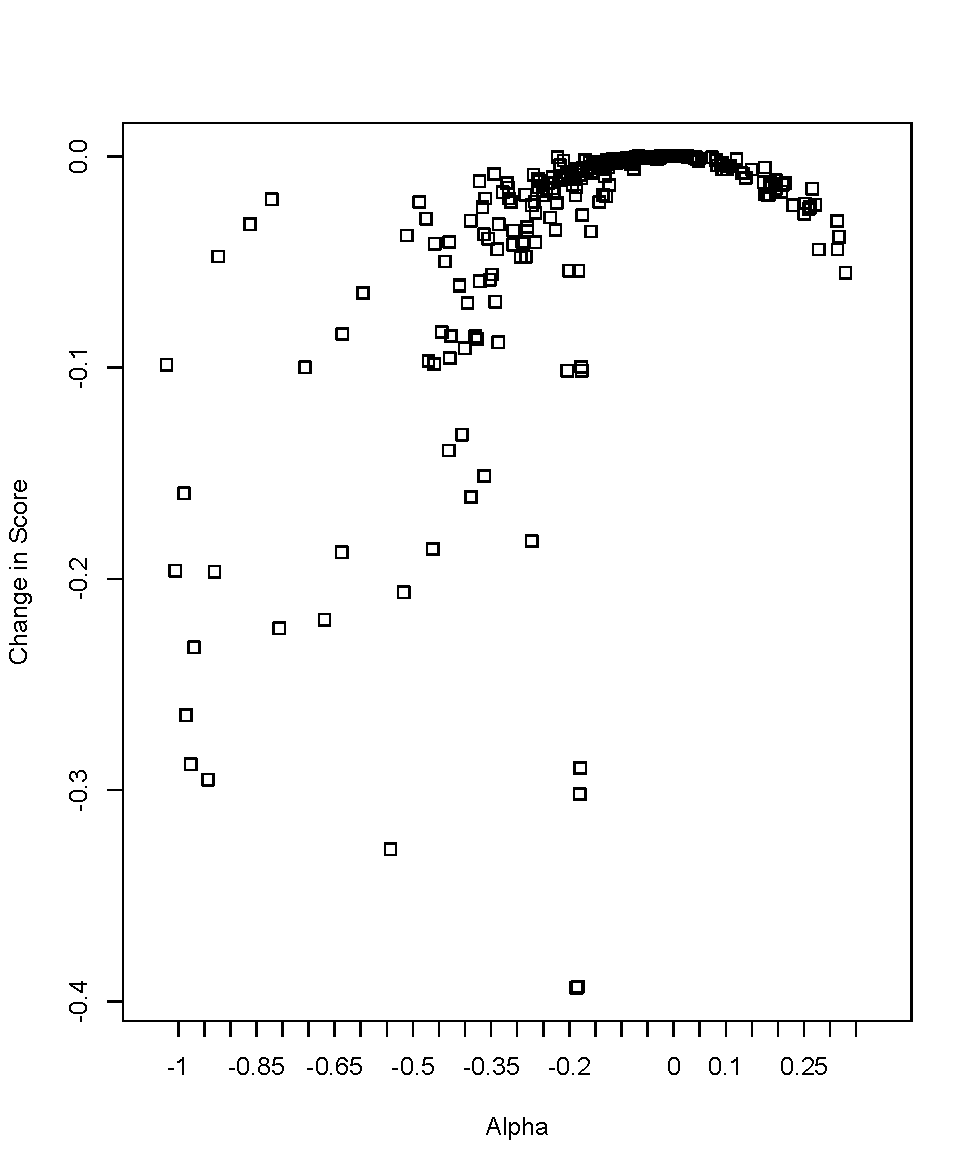
\includegraphics[width=\textwidth]{AlphaPlot.pdf}
	\caption{Kaggle team score improvements as a function of the $\alpha$ that would have maximized the scores.}
	\label{fig:alphas}
\end{figure}

The introduction of the parameter $\alpha$ to stretch or contract the estimated probabilities highlights the possibility that submitting values not equal to the actual probability estimates may be beneficial in some circumstances. To explore further, a Kaggle competitor may decide to specify a threshold, beyond which probabilities much larger (or smaller) than $0.5$ are pushed to $1$ (or $0$).

\section{Modeling}
This section details common prediction methods and then highlights our novel methodology that captures matchup specific factors.  As a means for motivation, consider claims of the type \emph{Team X is a tough matchup for team Y due to their ...} often made by sports broadcasters.  There are two ways to consider this statement: (i) the overall team strength of Team X will be problematic for Team Y or (ii) Team X has certain tendencies above and beyond their team strength that will pose difficulties for Team Y.  We outline a general framework for the first case, specifying models that account for differences in team strength.  However, for the second case a different approach is needed to analytically quantify characteristics that pose difficulties for a given team.  Many traditional methods, particularly those based on rankings, impose a characteristic we deem transitivity on predictions.  Our definition of transitivity is fully defined below, but the key point is that models with this property are inherently unable to capture problems of the second type.  We introduce the Nearest-Neighbor Matchup Effect which captures characteristics of specific match ups and doesn't adhere to transitivity in predictions.  

\subsection{Data Treatment}
For our purposes game summary data is used, but another approach not explored here focuses on simulating each sequence in a game rather than the complete outcome as in \cite{vstrumbelj2012}.  A few necessary considerations are whether the outcome of a game is binary (win/loss) or continuous (point differential) as well as whether linear or non-linear modeling (in the predictors) should be used.  The first interesting dilemma involves whether the outcomes should be modeled in a binary sense (win or loss) or rather should a continuous metric such as the point spread be used.  In theory, point spread provides a means for eliciting the relative strength of one team, although as any basketball fan can attest to the final score is often not indicative of how close the game was.  Nevertheless, point spreads are informative about the relative strength of one team compared to another.  Our experience showed that non-linear methods such as CART provided little extra predictive power when compared to linear methods.  \andyc{pull quote about simple models from Kaggle winners}

\subsection{Relative Strength Models}
Adopting the continuous treatment of game outcomes (e.g. point spread), the general form for the relative strength models follows below:
\begin{eqnarray}
Y_{ijk} = g_1(X_{ij}) + g_2(X_i) + g_3(X_j) +  \epsilon_{ijk}
\label{eq:RS}
\end{eqnarray}
where $X_{ij}$ corresponds to the difference in predictors for teams $i$ and $j$, $X_l$ contains predictors for team $l$, and $\epsilon_{ijk} \sim N(0,\sigma^2)$ corresponds to the $kth$ matchup between teams $i$ and $j$.  Most commonly $X_{ij}$ will consist of differences in rankings and seeds between the two teams.  A simple example for Equation~\ref{eq:RS} would be a simple linear model.

\subsection{Popular Methods}  This section provides a review of several existing methods for tournament prediction.
\subsubsection{Rating Based Methods} 
The seeds and ratings discussed earlier contain implicit or explicit means for tournament prediction.  For instance the Sagarin rankings are designed to reflect the point spread between two teams, incorporating a term for the variance of the outcomes under a Bayesian framework provides an efficient way to compute winning probabilities.  Similarly for any of the other rankings coefficients for predicting point spreads or in a binary regression can be computed. A seed based probability is shown in \cite{schwertman1996}.  A more sophisticated approach using point spreads along with Sagarin rankings is shown in \cite{carlin1996}.
\subsubsection{Ensemble Methods}
Combining the ratings from several different sites is a popular strategy.  In fact this is the technique used by Nate Silver's 538 methodology.  In particular Nate Silver's model incorporates ... \andyc{cite here}

\subsection{Nearest-Neighbor Matchup Effects}
The nearest-neighbor matchup effects are tailored for the second scenario posed in the introduction to this section in which there exist team level characteristics - above and beyond team strength - that contribute to win probability.  For instance, maybe a certain team struggles with taller teams that rebound well.  When facing an opponent with these attributes the team would expect to perform worse than the difference in team strengths would suggest.  Our procedure is a three step process: (i) fit a relative strength model of the form specified in Equation~\ref{eq:RS}, (ii) identify neighbors, by finding similarities between the current opponent and past opponents, and (iii) calibrate the matchup adjustment.  Fitting of the relative strength model follows the same form as previously described and will not be rehashed in this segment.
\subsubsection{Choosing Neighbors}
When choosing neighbors for a matchup between team $X$ and team $Y$, we need to identify past opponents of team $X$ with similar attributes to team $Y$ and past opponents of team $Y$ with similar attributes to team $X.$  The idea is to identify how the performance changes against that subset of opponents.

There are a multitude of ways to select the neighbors.  In particular one needs to consider what variables to consider for selecting neighbors, how should those variables be weighted if at all, and how many neighbors should be selected.  We consider a large set of team level data from which a 5-nearest neighbor approach is calculated.

Typically this procedure would be done analytically, however, user input can also be solicited.  For instance, suppose that a user decided Mercer was similar to Wake Forest and Clemson.  In this case current and ongoing work in Bayesian Visual Analytics (BAVA) framework detailed in \cite{house2010} provides a principled routine for visualizing teams and taking user input of similarities to create a method for computing distance between teams .  
\subsubsection{Matchup Adjustment}
The idea of the matchup adjustment is to quantify how much a team underperformed (or over performed) relative the expected level for a subset of teams similar to the current opponent.  So if team $i$ was two points better than expected against teams similar to $j$, then it would be reasonable to assume that team $i$ would perform better against team $j$ as well.  Assume a simple linear model is used for Equation \ref{eq:RS}, then the predictive distribution for a matchup between team $i$ and team $j$ now becomes 
\begin{eqnarray}
p(Y_{ij}|X_{ij}, \beta,\sigma^2,\mathcal{N}_i^k(j),\mathcal{N}_j^k(i), \rho) \sim N(X_{ij} \beta + \rho(\mathcal{N}_i^k(j) -\mathcal{N}_j^k(i)), \sigma^2),
\label{eq:ME}
\end{eqnarray}
where $\mathcal{N}_j^k(i)$ is the average residual for the team $i's$ $k$ past opponents most similar to team $j$ and $\rho$ is a tuning parameter $\in [0,1]$ that controls the amount of information passed from similar neighbors. 

The natural support of $\rho$ would be between zero and one.  The interpretation of the extreme points is rather intuitive - with $\rho = 0$ Equation~\ref{eq:ME} reverts to Equation~\ref{eq:RS} and with $\rho = 1$ the entire residual for similar teams is retained. 
\subsection{A note about Transitivity}
The transitive property states if $A>B$ and $B>C$ then $A>C$.   In terms of basketball prediction consider:
\begin{eqnarray}
P_{A,B} > 0.5 \quad \& \quad P_{B,C} > 0.5 \rightarrow P_{A,C} > 0.5
\label{eq:trans}
\end{eqnarray}
, where $P_{I,J}$ is the probability of team I defeating team J.  Then Equation \ref{eq:trans} can be considered a transitive property on basketball match ups.  That is if team A is expected to beat team B and team B is expected to beat team C, then team A should also defeat team C.  Any sort of rank based approaches would assume this transitive ordering, home court effects non-withstanding.  Note these are probabilities not true outcomes, due to the parity in basketball inferior teams can and often do defeat stronger teams.  On the other hand, our matchup effects modeling approach can determine if the strengths of a given team present difficulties for a specific team meaning the transitive property is not required to hold and $P_{A,B} > 0.5 \quad \& \quad P_{B,C} > 0.5\quad \& \quad P_{A,C} < 0.5$ is valid.

%\section{Model: Nearest-Neighbor Matchup Effects}
Sports broadcasters often make claims similar to \emph{Team X is a tough matchup for team Y due to their ... }.  There are two ways to consider this statement: (1) the overall team strength of Team X will be problematic for Team Y or (2) Team X has certain tendencies above and beyond their team strength that will pose difficulties for Team Y.  For the first case, models specified by Equation \ref{eq:generic} will account for differences in team strength.  However, for the second case a different approach is needed to analytically quantify characteristics that pose difficulties for a given team.  We introduce the Nearest-Neighbor Matchup Effect which captures characteristics of specific match ups.  For instance in hindsight, a glance inside the crystal ball would have revealed that Duke might struggle against Mercer.  It is not clear if this was the ten percent of instances that a 14 seed defeats a 3 seed, \andyc{check this historical frequency} or whether an uncharacteristically difficult matchup to the Mercer's characteristics for third seeded Duke.  Perhaps an astute observer - or clustering algorithm - would have recognized that Mercer was a team with similar characteristics to Clemson and Wake Forest, two teams Duke struggled against during the regular season. Then the matchup effect would have revised to initial probability of Duke winning to account for the fact that Mercer has similar characteristics to Clemson and Wake Forest resulting in a winning probability of 72 percent compared to the initial 90 percent estimate.  Computing matchup effects is a three step procedure: (1)  the typical model as in Equation~\ref{eq:generic} is fit, (2) for each matchup, past opponents most similar to the current matchup are identified, and (3) an adjustment is introduced that accounts for past performance against similar teams. 
\subsection{Relative Strength Models}
The general form for the relative strength models follows below:
\begin{eqnarray}
Y_{ij} = X_{ij} \beta + \epsilon
\label{eq:ME}
\end{eqnarray}
where $X_{ij}$ coresponds to the difference in predictors for teams $i$ and $j.$  Most commonly $X_{ij}$ will consist of differences in rankings and seeds between the two teams. 

\subsection{Choosing Neighbors}
There are a multitude of ways to select the neighbors.  In particular one needs to consider what variables to consider for selecting neighbors, how should those variables be weighted if at all, and how many neighbors should be selected.  We consider a large set of team and player level data from which a k-nearest neighbor approach is calculated.

Typically this procedure would be done analytically, however, user input can also be solicited.  For instance, suppose as in the earlier example that a user decided Mercer was similar to Wake Forest and Clemson.  In this case, Bayesian Visual Analytics (BAVA) provides a principled routine for visualizing teams and specify similarities.
\subsection{Matchup Adjustment}
The idea of the matchup adjustment is to quantify how much a team underperformed (or over performed) relative the expected level for a subset of teams similar to the current opponent.  So if team $i$ was two points better than expected against teams similar to $j$, then it would be reasonable to assume that team $i$ would perform better against team $j$ as well.  Then the predictive distribution for a matchup between team $i$ and team $j$ now becomes
\begin{eqnarray}
p(Y_{ij}|X_{ij}, \beta,\sigma^2,\mathcal{N}_i^k(j),\mathcal{N}_j^k(i), \rho) \sim N(X_{ij} \beta + \rho(\mathcal{N}_i^k(j) -\mathcal{N}_j^k(i)), \sigma^2),
\label{eq:ME}
\end{eqnarray}
where $\mathcal{N}_j^k(i)$ is the average residual for the team $i's$ $k$ past opponents most similar to team $j$ and $\rho$ is a tuning parameter $\in [0,1]$ that controls the amount of information passed from similar neighbors. 
\subsection{Tuning $\rho$}
The natural support of $\rho$ would be between zero and one.  The interpretation of the extreme points is rather intuitive - with $\rho = 0$ Equation~\ref{eq:ME} reverts to Equation~\ref{eq:generic} and with $\rho = 1$ the entire residual for similar teams is retained.  For our analysis, we choose the $\rho$ value that optimized the mean risk in previous years.  Comprehensive team level characteristics are available going back seven years, so for the 2014 tournament we chose $\rho=0.2$.

\section{Evaluation}
To demonstrate the efficacy of our method, we first fit Equation~\ref{eq:RS} using a well known rating system, the Sagarin ratings.  Then, $\rho$ is calibrated based on historical results from the previous seven years NCAA tournaments.  Note seven years was chosen as this is the complete history of the team and player level characterstics used to find neighbors of teams.   The log loss for 2014 for the entire range of $\rho$ can be seen in Figure~\ref{fig:result} and the value that was selected based on historical results $0.2$.
\begin{figure}[h]
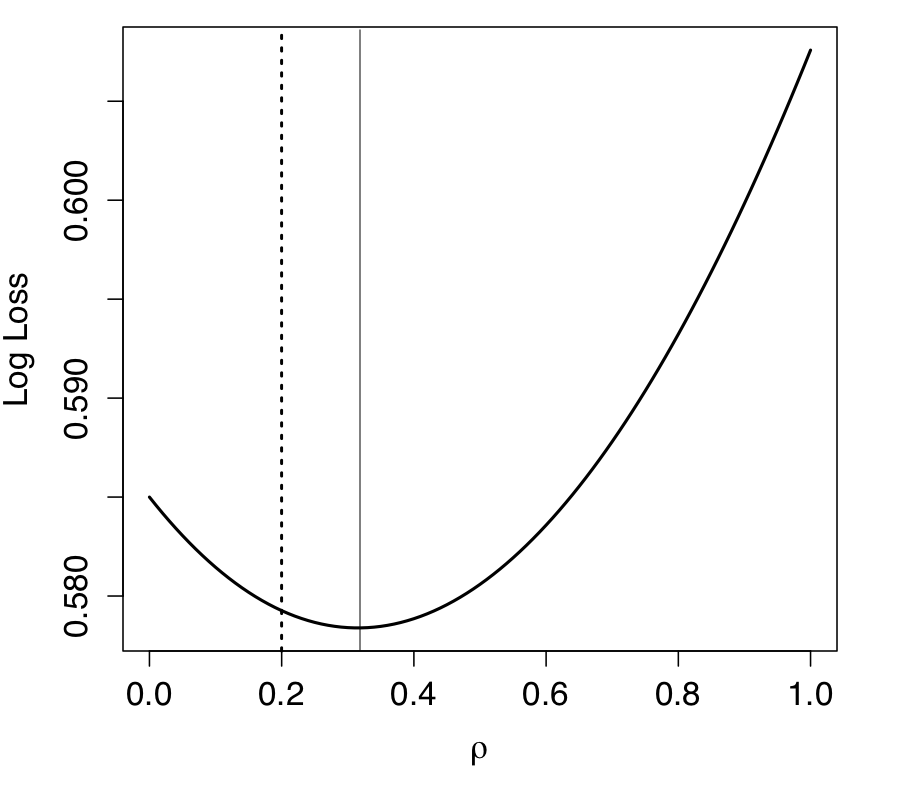
\includegraphics[width=1\textwidth]{results_2014.png}
\caption{Log loss for no matchup effect = red, log loss for optimized $\rho$ = blue}
\label{fig:result}
\end{figure}

The selected $\rho$ value results in a reduction in loss.  A modest gain is also seen in classification error from (0.365 to 0.350) although this is only a single game difference.  The matchup effect, particularly with smaller $\rho$ values, will have a lesser effect on classification error than that off the loss functions like the log loss.  This is because it will only shift the expected point differential a fairly small margin, so the only games in which classification error would change are those that are nearly dead heat games to begin with.

To illustrate the matchup effects, consider Table~\ref{tab:change} which contains the ten games that saw the largest shift in expected point differential.  This table contains expected point differentials (team1 - team2) and probabilities of team 1 winning under a standard relative strength model using the Sagarin ratings as well as the adjusted results using the Nearest Neighbor Matchup Effects.  The table also contains the realized loss for the each resulting game.
\begin{table}[ht]
\caption{Ten games with largest point differential change}
\footnotesize
\centering
\begin{tabular}{|cc | ccc | ccc | c|}
  \hline
  \hline
 team 1 & team 2 & Point Diff & Prob & Loss & Point Diff:ME & Prob:ME & Loss:ME & winning team \\ 
  \hline
 Cal Poly & Wichita St & -18.69 & 0.04 & 0.04 & -17.10 & 0.06 & 0.06 & Wichita St \\ 
 Connecticut & St. Joseph's &4.29 & 0.65 & 0.43 & 6.18 & 0.71 & 0.34 & Connecticut \\ 
 Dayton & Stanford & -2.16 & 0.42 & 0.86 & 0.94 & 0.53 & 0.63 & Dayton \\ 
 Dayton & Syracuse & -6.34 & 0.28 & 1.27 & -4.05 & 0.36 & 1.03 & Dayton \\ 
 Kentucky & Michigan & -3.71 & 0.37 & 1.00 & -2.08 & 0.42 & 0.86 & Kentucky \\ 
 UMass & Tennessee &-3.05 & 0.39 & 0.49 & -4.83 & 0.33 & 0.40 & Tennessee \\ 
 Memphis & Virginia & -6.34 & 0.28 & 0.33 & -8.91 & 0.21 & 0.23 & Virginia  \\ 
 Michigan & Tennessee & 5.37 & 0.69 & 0.37 & 3.49 & 0.62 & 0.47 & Michigan\\ 
 Michigan & Texas & 8.05 & 0.77 & 0.26 & 5.85 & 0.70 & 0.35 & Michigan \\ 
 Syracuse & W. Michigan & 12.65 & 0.88 & 0.13 & 15.01 & 0.92 & 0.09 & Syracuse \\ 
   \hline
   \hline
\end{tabular}
\label{tab:change}
\end{table}
On this particular subset of games, the matchup effects model performs considerably better than the typical model under the log loss (.446 to .520).  As the other games see minimal matchup effects, the results are essentially the same.  
\section{Luck}
how sensitive is the leader board. It's natural to think 2nd place almost won, but how close was 20th place to winning. (Lucas: sensitivity study)

\section{Inference on Transitivity}
\andyc{This may get cut}
The transitive property states if $A>B$ and $B>C$ then $A>C$.   In terms of basketball consider:
\begin{eqnarray}
P_{A,B} > 0.5 \quad \& \quad P_{B,C} > 0.5 \rightarrow P_{A,C} > 0.5
\label{eq:trans}
\end{eqnarray}
, where $P_{I,J}$ is the probability of team I defeating team J.  Then Equation \ref{eq:trans} can be considered a transitive property on basketball match ups.  That is if team A is expected to beat team B and team B is expected to beat team C, then team A should also defeat team C.  Any sort of rank based approaches would assume this transitive ordering, home court effects non-withstanding.  Note these are probabilities not true outcomes, due to the parity in basketball inferior teams can and often do defeat stronger teams.  Nevertheless, our modeling approach can determine if the strengths of a given team present difficulties for a specific team resulting in the transitive property not necessarily holding.

\section{Recommendations}
In general NCAA bracket competitions, \cite{niemi2008} and \cite{breiter1997} provide a good overview of optimal strategies.  As probabilistic predictions are a bit different we highlight some high level ideas and then provide more detailed recommendations. Our takeaway from this competition is that high quality data, reasonable models, and a little luck are the components for a successful modeling competition. This is echoed by \cite{kaggle}, the winning Kaggle competitors.
\begin{quote}
Q: Were you surprised by any of your insights?

Greg: I was surprised by how well our simple models performed. Using the right data was MUCH more important to our models performing well than using more sophisticated models.

Mike: I think we gave ourselves a chance with a good model, but there was probably a decent amount of luck involved, too. Also, identifying the specific loss function for this Kaggle contest, and where it comes from, seemed to help our model.
\end{quote}
We also found that there seemed to be little advantage in using complex models as simple linear models worked quite well.  Something that was beneficial was modeling point spread rather than treating wins and losses in a binary sense, this agrees with  \cite{gelman}:
\begin{quote}
Don't model the probability of win, model the expected score differential. Yeah, I know, I know, what you really want to know is who wins. But the most efficient way to get there is to model the score differential and then map that back to win probabilities. The exact same issue comes up in election modeling: it makes sense to predict vote differential and then map that to Pr(win), rather than predicting Pr(win) directly. This is most obvious in very close games (or elections) or blowouts; in either of these settings the win/loss outcome provides essentially zero information. But it's true more generally that there's a lot of information in the score (or vote) differential that�s thrown away if you just look at win/loss.
\end{quote}
Next we provide more detailed strategies for probabilistic modeling competitions.
\subsection{Optimal Strategies}
\andyc{Marcos's piece here}
How should a typical user use this to figure out their bracket/Kaggle competition?
\section{Discussion}
As shown in the the section on luck, chance coupled with a relatively small sample size makes winning NCAA prediction competitions a difficult task.  Nevertheless, we provide some sound methods and techniques for making game-by-game predictions. Our matchup effects model is an intuitive means for adjusting probabilities based on matchup specific characteristics. While there undoubtably is a more principled way to carry out this exercise, and given the time constraints, we found this to be effective.

Other considerations would be to use injury data for players as Nate Silver's 538.com does. However, this particular competition required predictions for the complete tournament in advance of the first games. Nevertheless, knowing the status of Kansas's Joel Embiid would have shifted probabilities for Kansas and similarly the effect of Iowa State's Georges Niang injury prior to the sweet sixteen matchup with Connecticut would undoubtedly have lead to different predictive values

Something else that may be beneficial would be to use the score with two minutes to go, for example, to quantify how a game was. As any fan can attest, the strategy of fouling can lead to dramatically different scores as can garbage time minutes by reserves, which results in a distorted view of how close the game was. However, the time constraints for this year's competition deterred us from pursuing this - perhaps next year.


%%%%%%%%%%%%%%%%%%%%%%%%%%%%%%%%%%%%%%%%%%%
%%%%%%%%%%%%%%%%%%%%%%%%%%%%%%%%%%%%%%%%%%%
%%%%%%%%%%%%%%%%%%%%%%%%%%%%%%%%%%%%%%%%%%%

\marcosc{hmm...}
\cite{Gelman}

\bibliographystyle{asa}
\bibliography{refsJQAS}

%%%%%%%%%%%%%%%%%%%%%%%%%%%%%%%%%%%%%%%%%%%
%%%%%%%%%%%%%%%%%%%%%%%%%%%%%%%%%%%%%%%%%%%

%%%%%%%%%%%%%%%%%%%%%%%%%%%%%%%%%%%%%%%%%%%


%%%%%%%%%%%%%%%%%%%%%%%%%%%%%%%%%%%%%%%%%%%

\end{document}
